\begin{figure}[H]
\centering
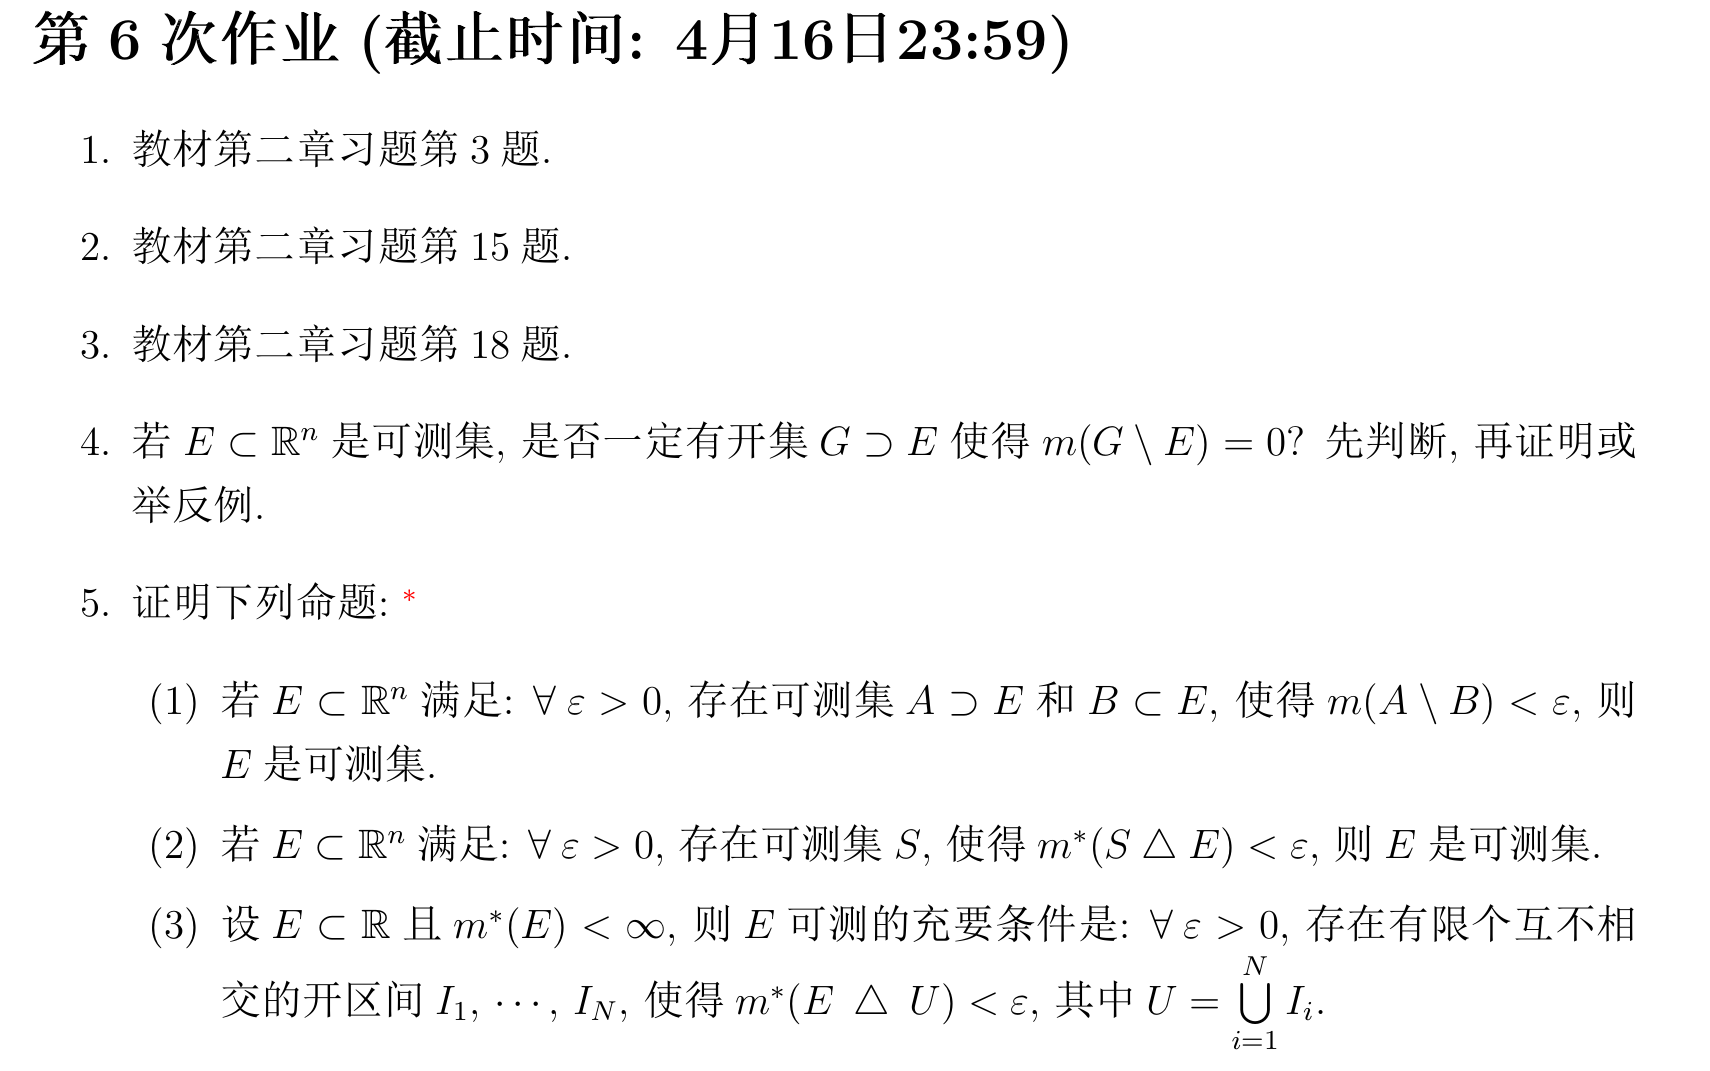
\includegraphics[width=\textwidth]{hw6-2025041520.png}
% \caption{}
\label{}
\end{figure}
\begin{figure}[H]
\centering
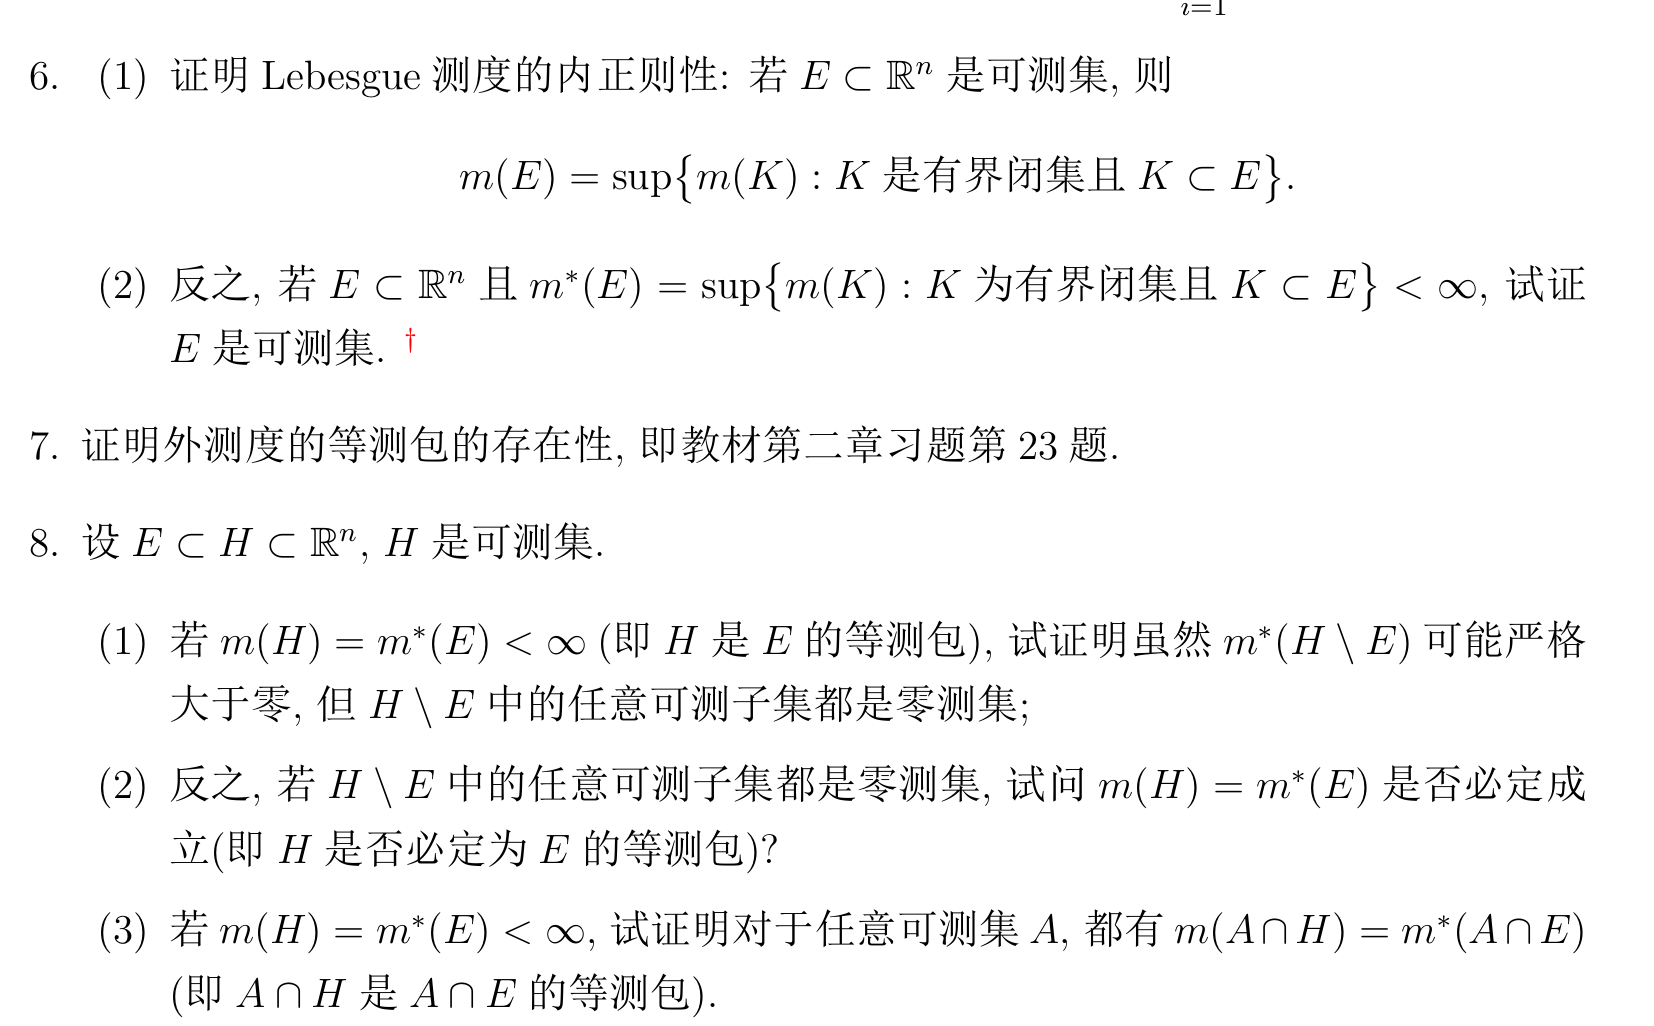
\includegraphics[width=\textwidth]{1-hw6-2025041520.png}
% \caption{}
\label{}
\end{figure}
\begin{figure}[H]
\centering
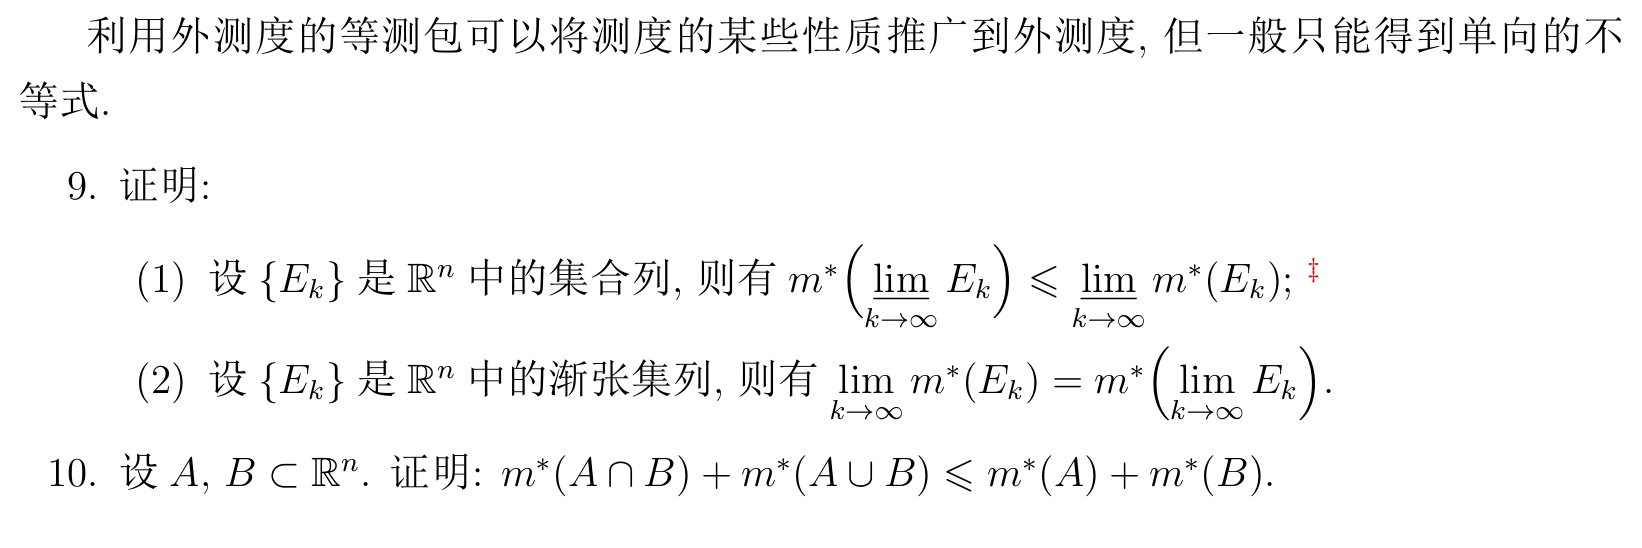
\includegraphics[width=\textwidth]{2-hw6-2025041520.png}
% \caption{}
\label{}
\end{figure}

\begin{exercise}
设 $E \subset[0,1]$ 为可测集,若 $m E=1$ ,试证 $\overline{E}=[0,1]$ ;若 $m E=0$ ,试证 $E^o=\varnothing$ .
\end{exercise}
\begin{proof}
反证而设, $\overline{E}\neq[0,1]$,则存在 $x\in[0,1]$,$x$ 并非 $E$ 的聚点,故存在区间 $I_{x}=I_{x}\cap [0,1]$ 使得 $x\in I_{x},I_{x}\cap E=\varnothing$. 故 $E\subset[0,1]\setminus I_{x}$,$1=mE\leq 1-mI_{x}<1$ 矛盾!

若 $E^{o}\neq \varnothing$,则对于 $p\in E^{o}$,存在 $p$ 的邻域(某个区间)$I_{p}=I_{p}\cap [0,1]$,使得 $I_{p}\subset E$,于是 $0=mE\geq mI_{p}>0$ 矛盾!
\end{proof}

\begin{exercise}
\begin{figure}[H]
\centering
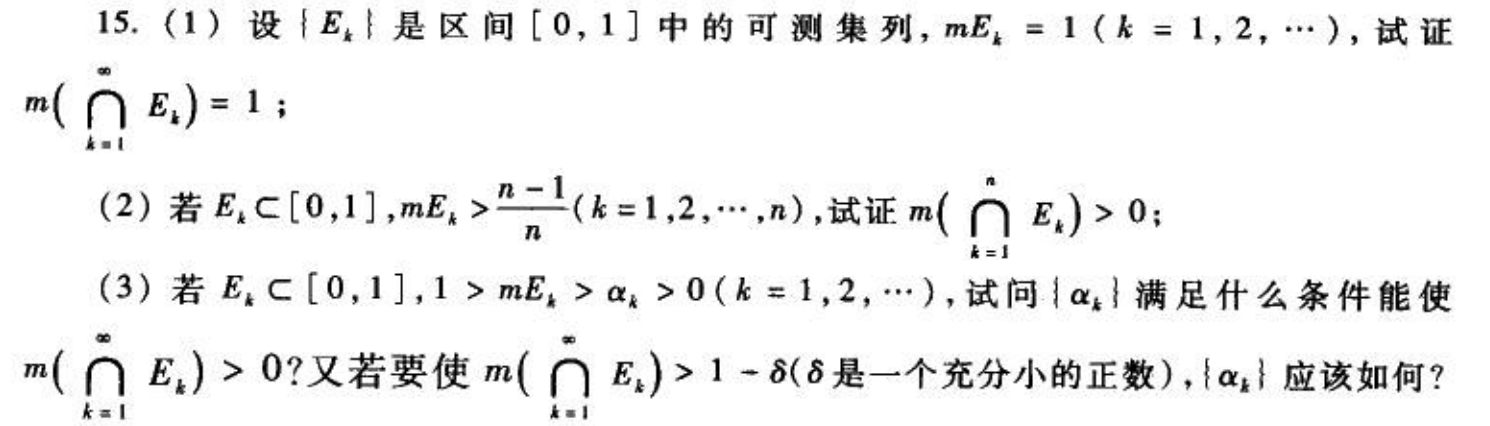
\includegraphics[width=\textwidth]{hw6-2025041600.png}
% \caption{}
\label{}
\end{figure}
\end{exercise}
\begin{proof}
(1)
\[
\begin{aligned}
m\left( \bigcap_{k=1}^{\infty} E_k \right) & =1-m\left( [0,1]\setminus\left( \bigcap_{k=1}^{\infty} E_k \right) \right) \\
 & =1-m\left( \bigcup_{k=1}^{\infty} ([0,1]\setminus E_k) \right) \\
 & \geq 1-\sum_{k=1}^{\infty} m([0,1]\setminus E_k) \\
 & =1-\sum_{k=1}^{\infty} (\underbrace{ 1-mE_k }_{ =0 }) \\
 & =1
\end{aligned}
\]
又因为
\[
m\left( \bigcap_{k=1}^{\infty} E_k \right)\leq m(E_1)
\]
故
\[
m\left( \bigcap_{k=1}^{\infty}  E_k\right)=1
\]
(2)
\[
\begin{aligned}
m\left( \bigcap_{k=1}^{n} E_k \right) & =1-m\left( [0,1]\setminus\left( \bigcap_{k=1}^{n} E_k \right) \right) \\
 & =1-m\left( \bigcup_{k=1}^{n} ([0,1]\setminus E_k) \right) \\
 & =1-\sum_{k=1}^{n} m([0,1]\setminus E_k) \\
 & =1-\sum_{k=1}^{n} (1-mE_k) \\
 & >1-\sum_{k=1}^{n} \left( 1-\frac{n-1}{n} \right) \\
 & =0
\end{aligned}
\]
(3)
\[
\begin{aligned}
m\left( \bigcap_{k=1}^{n} E_k \right) & =1-m\left( [0,1]\setminus\left( \bigcap_{k=1}^{n} E_k \right) \right) \\
 & =1-m\left( \bigcup_{k=1}^{n} ([0,1]\setminus E_k) \right) \\
 & =1-\sum_{k=1}^{n} m([0,1]\setminus E_k) \\
 & =1-\sum_{k=1}^{n} (1-mE_k) \\
 & >1-\sum_{k=1}^{n} \left( 1-\alpha _k \right) \\
 & =1-n+\sum_{k=1}^{n} \alpha _k
\end{aligned}
\]
要使得 $m\left( \bigcap_{k=1}^{n}E_k \right)>0$ 只需要 $\sum_{k=1}^{n}\alpha _k>n-1$.

要使得 $m\left( \bigcap_{k=1}^{n}E_k \right)>1-\delta$ 只需要 $\sum_{k=1}^{n}\alpha _k>n-\delta$.
\end{proof}

\begin{exercise}
\begin{figure}[H]
\centering
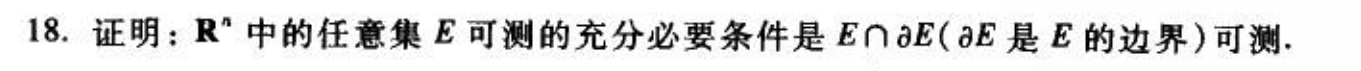
\includegraphics[width=\textwidth]{1-hw6-2025041600.png}
% \caption{}
\label{}
\end{figure}
\end{exercise}
\begin{note}
开集和闭集的边界可能有正测度!
\end{note}
\begin{proof}
记

\begin{itemize}
	\item $\operatorname{Int}(E)$ 为 $E$ 的内点集;
	\item $\partial E$ 为 $E$ 的边界, 则
\end{itemize}
\[
\partial E = \overline{E} \setminus \operatorname{Int}(E).
\]
\textbf{必要性} (若 $E$ 可测, 则 $E \cap \partial E$ 可测):

\begin{enumerate}
	\item $\operatorname{Int}(E)$ 是开集, 故可测;
	\item $\overline{E}=\mathbb{R}^n \setminus \operatorname{Int}\left(E^c\right)$, 其中 $\operatorname{Int}\left(E^c\right)$ 是开集、可测, 所以 $\overline{E}$ 也是可测;
	\item $\partial E=\overline{E} \setminus \operatorname{Int}(E)$ (两可测集之差) 可测;
	\item 因此 $E \cap \partial E$ (两可测集之交) 可测。
\end{enumerate}

\textbf{充分性} (若 $E \cap \partial E$ 可测, 则 $E$ 可测):
\[
E=\operatorname{Int}(E) \cup(E \cap \partial E),
\]
其中 $\operatorname{Int}(E)$ 是可测的开集, $E \cap \partial E$ 假设可测, 故二者并集 $E$ 可测。

综上所述, 任意 $E \subset \mathbb{R}^n$ 可测当且仅当 $E \cap \partial E$ 可测。
\end{proof}

\begin{exercise}
\begin{figure}[H]
\centering
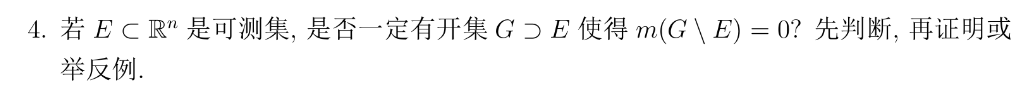
\includegraphics[width=\textwidth]{2-hw6-2025041600.png}
% \caption{}
\label{}
\end{figure}
\end{exercise}
\begin{proof}
不一定. 当 $n=1$,考虑 $E=\mathbb{Q}\cap[0,1]$,显然 $m^{*}E=0$,故 $E$ 可测,$mE=0$,对于任意包含 $E$ 的开集 $G$,对于任意 $x\in E\subset G$,$x$ 的某个充分小小邻域都在 $G$ 内,由于 $E$ 在 $[0,1]$ 内稠密,故对于充分小的 $\epsilon_{x}>0$,$B_{x}(\epsilon_{x})\subset G$,从而
\[
[0,1]\subset \bigcup_{x\in E}^{}B(x,\epsilon_{x})\subset G
\]
于是
\[
[0,1]\setminus \mathbb{Q}=[0,1]\setminus E\subset G\setminus E
\]
故
\[
m(G\setminus E)\geq m([0,1]\setminus Q)=1
\]
\end{proof}

\begin{exercise}
\begin{figure}[H]
\centering
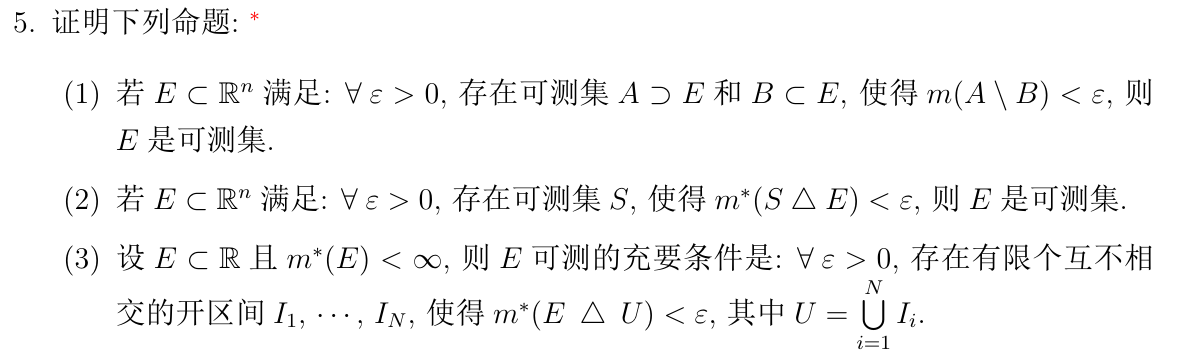
\includegraphics[width=\textwidth]{3-hw6-2025041600.png}
% \caption{}
\label{}
\end{figure}\label{5c15b8}
\end{exercise}

\begin{proof}
(1) 只需要验证对于任意集合 $C\subset \mathbb{R}^{n}$,满足
\[
m^{*}C\geq m^{*}(C\cap E)+m^{*}(C\cap E^{c})
\]
我们知道 $C\cap E\subset C\cap A,C\cap E^{c}\subset C\cap B^{c}$. 于是
\[
m^{*}(C\cap E)\leq m^{*}(C\cap A),\qquad m^{*}(C\cap E^{c})\leq m^{*}(C\cap B^{c})
\]
又因为
\[
\begin{aligned}
C & =(C\cap A^{c})\cup(C\cap A) \\
 & \subset(C\cap A^{c})\cup(C\cap((A\setminus B)\cup B)) \\
 & \subset(C\cap A^{c})\cup(C\cap(A\setminus B))\cup(C\cap B) \\
 & \subset(C\cap A^{c})\cup(C\cap B)\cup(A\setminus B)
\end{aligned}
\]
故
\[
\begin{aligned}
m^{*}(C\cap E)+m^{*}(C\cap E^{c}) & \leq m^{*}(C\cap A)+m^{*}(C\cap B^{c}) \\
 & =m^{*}C-m^{*}(C\cap A^{c})+m^{*}C-m^{*}(C\cap B) \\
 & \leq m^{*}(C\cap A^{c})+m^{*}(C\cap B)+m^{*}(A\setminus B)-m^{*}(C\cap A^{c}) \\
 &\qquad +m^{*}C-m^{*}(C\cap A^{c}) \\
 & =m^{*}C+m^{*}(A\setminus B) \\
 & <m^{*}C+\epsilon
\end{aligned}
\]
由 $\epsilon$ 任意性,$m^{*}(C\cap E)+m^{*}(C\cap E^{c})\leq m^{*}C$. 因此 $E$ 可测.

(2) 只需要验证对于任意集合 $C\subset \mathbb{R}^{n}$,满足
\[
m^{*}C\geq m^{*}(C\cap E)+m^{*}(C\cap E^{c})
\]
因为
\[
C\cap E\subset C\cap(S\cup(E\setminus S))=(C\cap S)\cup(C\cap(E\setminus S))\subset(C\cap S)\cup(E\setminus S)
\]
\[
\begin{aligned}
C\cap E^{c} & \subset C\cap(S\cap E)^{c}=C\cap(S^{c}\cup E^{c})=C\cap(S^{c}\cup(E^{c}\setminus S^{c})) \\
 & =C\cap(S^{c}\cup(E^{c}\cap S)) \subset (C\cap S^{c})\cup(C\cap E^{c}\cap S) \\
 & =(C\cap S^{c})\cup(C\cap(S\setminus E))\subset(C\cap S^{c})\cup(S\setminus E)
\end{aligned}
\]
所以
\[
\begin{aligned}
m^{*}(C\cap E)+m^{*}(C\cap E^{c}) & \leq m^{*}(C\cap S)+m^{*}(E\setminus S)+m^{*}(C\cap S^{c})+m^{*}(S\setminus E) \\
 & =m^{*}C+m^{*}(\underbrace{ (E\setminus S)\cup(S\setminus E) }_{ =E\Delta S }) \\
 & <m^{*}C+\epsilon
\end{aligned}
\]
由 $\epsilon$ 任意性,
\[
m^{*}(C\cap E)+m^{*}(C\cap E^{c})\leq m^{*}C
\]
故 $E$ 可测.

(3) 充分性由 (2) 显然,下面证明必要性.

假设 $E$ 可测,则对于任意给定的 $\epsilon>0$,可作开集 $G=\bigcup_{i=1}^{\infty}I_i\supset E$ 且 $m(G\setminus E)<\epsilon$, 从而
\[
m^{*}\left( \bigcup_{i=1}^{n_0} I_i\setminus E \right)\leq m^{*}\left( \bigcup_{i=1}^{\infty} I_i\setminus E \right)=m^{*}(G\setminus E)<\epsilon
\]
此外
\[
\left( E\setminus \bigcup_{i=1}^{n_0} I_i \right)\subset \bigcup_{i=n_0+1}^{\infty} I_i\implies m\left( E\setminus \bigcup_{i=1}^{n_0} I_i \right)\leq  m\left( \bigcup_{i=n_0+1}^{\infty} I_i \right)
\]
取 $n_0$ 充分大使得
\[
m\left( \bigcup_{i=n_0+1}^{\infty} I_i \right)<\epsilon
\]
于是
\[
m\left( E\Delta \bigcup_{i=1}^{n_0} I_i \right)\leq m\left( E\setminus \bigcup_{i=1}^{n_0} I_i \right)+m\left( \bigcup_{i=1}^{n_0} I_i\setminus E \right)<2\epsilon
\]
得证!
\end{proof}

\begin{exercise}
\begin{figure}[H]
\centering
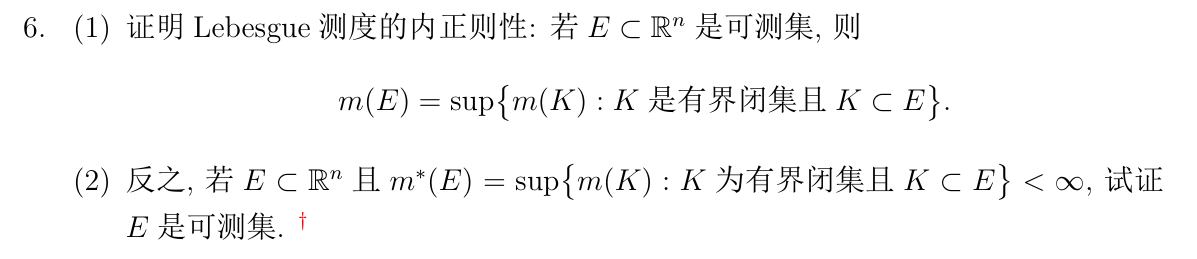
\includegraphics[width=\textwidth]{hw6-2025041601.png}
% \caption{}
\label{}
\end{figure}
\end{exercise}
\begin{proof}

\begin{lemma}
\begin{figure}[H]
\centering
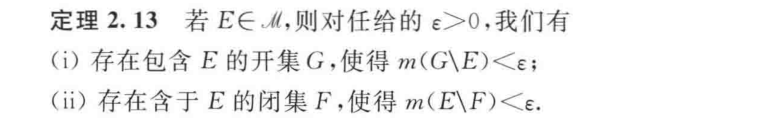
\includegraphics[width=\textwidth]{1-hw6-2025041608.png}
% \caption{}
\label{}
\end{figure}\label{336926}
\end{lemma}

\begin{proof}
若 $mE<\infty$,根据可测的定义,存在一列开区间 $\{ I_k \}_{k=1}^{\infty}$ , 使得 $E\subset \bigcup_{k=1}^{\infty}I_k\eqqcolon G$ (开集的任意并还是开集),且
\[
mE\geq \sum_{k=1}^{\infty } l(I_k)-\epsilon
\]
于是
\[
mG\leq \sum_{k=1}^{\infty} l(I_k)\leq mE+\epsilon
\]
于是
\[
m(G\setminus E)=mG-mE\leq \epsilon
\]
若 $m^{*}E=\infty$,定义 $E_k=E\cap B(0,k)$ (有限测度),则对于任意给定的 $\epsilon>0$, 存在开集 $G_k$ 使得
\[
m(G_k\setminus E_k)\leq \frac{\epsilon}{2^{k}}
\]
那么定义 $G=\bigcup_{k=1}^{\infty }G_k$ (仍然是开集),则
\[
\begin{aligned}
m(G\setminus E) & =m\left( \bigcup_{k=1}^{\infty} (G_k \setminus E) \right) \\
 & \leq m\left( \bigcup_{k=1}^{\infty} G_k\setminus E_k \right) \\
 & \leq \sum_{k=1}^{\infty} m(G_k\setminus E_k) \\
 & \leq \sum_{k=1}^{\infty} \frac{\epsilon}{2^{k}} \\
 & =\epsilon
\end{aligned}
\]
故得证!

接下来对于集合 $E$,考虑 $E^{c}$,对于任意给定的 $\epsilon>0$,存在开集 $G\supset E^{c}$,使得 $m(G\setminus E^{c})<\epsilon$. 现在令 $F\coloneqq G^{c}$,由于 $E\setminus F=G\setminus E^{c}$,所以 $m (E\setminus F)=m(G\setminus E^{c})<\epsilon$. 故得证!
\end{proof}

(1)
若 $mE$ 有限,只需要证明:若 $E\subset \mathbb{R}^{n}$ 可测,那么对于任意给定的 $\epsilon>0$,存在有界闭集 $K\subset E$,使得
\[
m(K)\geq m(E)-\epsilon
\]
也就是
\[
m^{*}(E\setminus K)\leq \epsilon
\]
对于任意给定的 $\epsilon>0$,存在 $R>0$,使得 $m(E\setminus  \overline{B(0,R)} )<\frac{\epsilon}{2}$. 由 \cref{336926} 可知,存在闭集 $K$,使得
\[
m((E\cap  \overline{B(0,R)})\setminus K)< \frac{\epsilon}{2}
\]
由于
\[
\begin{aligned}
E\setminus K & =((E\cap  \overline{B(0,R)})\cup(E\setminus  \overline{B(0,R)}))\setminus K \\
 & =((E\cap  \overline{B(0,R)})\setminus K)\cup((E\setminus  \overline{B(0,R)})\setminus K) \\
 & \subset((E\cap  \overline{B(0,R)})\setminus K)\cup(E\setminus   \overline{B(0,R)})
\end{aligned}
\]
于是
\[
m^{*}(E\setminus K)\leq m^{*}((E\cap  \overline{B(0,R)})\setminus K)+m^{*}(E\setminus  \overline{B(0,R)})\leq \frac{\epsilon}{2}+\frac{\epsilon}{2}=\epsilon
\]
若 $m^{*}E=\infty$,那么定义 $E_m=E\cap \overline{B(0,m)}$,于是
\[
E=\bigcup_{m=1}^{\infty} E_m
\]
由于 $m^{*}E_m<\infty$,那么根据 \cref{336926} ,存在 $K_m\subset E_m\subset E$,使得 $m^{*}K_m+1\geq m^{*}E_m\to \infty$,于是
\[
\sup \{ m(K):K\text{ 为有界闭集且 }K\subset E \}=+\infty=mE
\]
(2) 由 \cref{336926} 可知,对于任意给定的 $\epsilon>0$ 存在包含 $E$ 的开集 $\mathcal{O}$,使得 $m(\mathcal{O}\setminus E)<\frac{\epsilon}{2}$.

与此同时,$m^{*}(E)=\sup \{ m(K):K\text{ 为有界闭集且 }K\subset E \}<\infty$,从而存在有界闭集 $K$ ,使得
\[
m^{*}E\leq m(K)+\frac{\epsilon}{2}
\]
从而 $K\subset E\subset \mathcal{O}$,且 $m^{*}\mathcal{O}-m^{*}K\leq\epsilon$. 由 \cref{5c15b8} (1) 可知 $E$ 可测.

\end{proof}

\begin{exercise}
\begin{figure}[H]
\centering
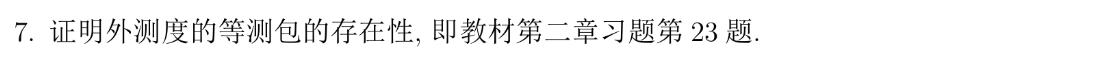
\includegraphics[width=\textwidth]{hw6-2025041608.png}
% \caption{}
\label{}
\end{figure}
\end{exercise}
\begin{proof}
由 \cref{336926} 可知,对于任意 $k\geq1$,存在集合 $G_k\supset E$ 使得
\[
mG_{k}\leq m^{*}E+\frac{1}{k}
\]
记 $H=\bigcap_{k=1}^{\infty}G_k\supset E$,那么 $H$ 是 $G_{\delta}$ 集,且
\[
m^{*}E\leq mH\leq m(G_k)\leq m^{*}E+\frac{1}{k},\qquad \forall k\geq 1
\]
令 $k\to \infty$,那么 $m^{*}E=mH$,且 $E\subset H$. $H$ 是 $E$ 的等测包,存在!
\end{proof}

\begin{exercise}
\begin{figure}[H]
\centering
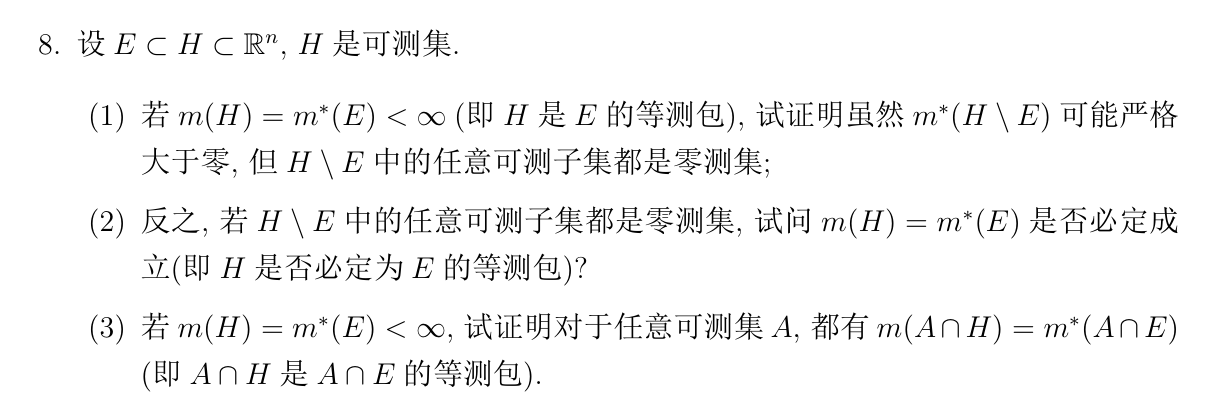
\includegraphics[width=\textwidth]{hw6-2025041609.png}
% \caption{}
\label{}
\end{figure}\label{0e7d37}
\end{exercise}

\begin{proof}

\begin{lemma}[From Royden]
\begin{figure}[H]
\centering
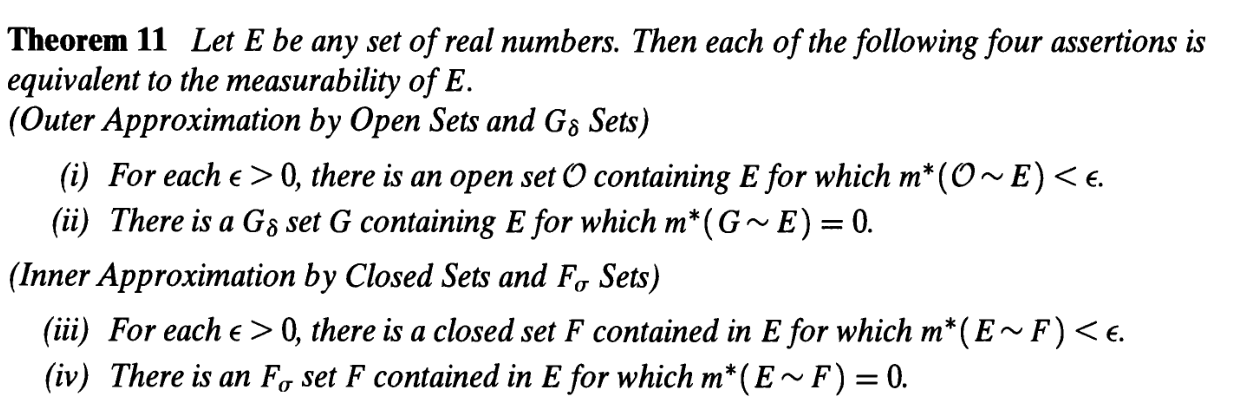
\includegraphics[width=\textwidth]{1-hw6-2025041609.png}
% \caption{}
\label{}
\end{figure}
\end{lemma}
(1)
$m^{*}(H\setminus E)$ 确实可能严格大于零,因为 $E$ 不一定可测,而 $m^{*}(H\setminus E)=0$ 等价于 $E$ 可测. 该等价性的证明如下:
\[
E=H\setminus(H\setminus E)
\]
其中 $H$ 可测,$m^{*}(H\setminus E)=0$ 由于零外测集一定可测,所以 $H\setminus E\in \mathcal{M}$,由于 $H\in \mathcal{M}$,所以 $E\in \mathcal{M}$. 反之,若有 $E$ 可测,则根据 \cref{336926} 可知,存在 $H\supset E$,$H\in G_{\delta}$,使得 $m^{*}(H\setminus E)=0$.

接下来考虑 $H\setminus E$ 的任意可测子集 $A$,有 $A\cap E=\varnothing$,由于 $E\subset H$,那么 $E\subset H\setminus A\subset H$. 由于 $A, H\in \mathcal{M}$,所以 $H\setminus A\in \mathcal{M}$. 由于 $m^{*}(E)=mH$,所以 $m^{*}(H\setminus A)=mH$,由于 $H\setminus A\in \mathcal{M}$,于是
\[
mA=m(H\setminus(H\setminus A))=m^{*}(H\setminus(H\setminus A))=0
\]
(2) 作 $E$ 的等测包 $G$,于是 $H\setminus G\subset H\setminus E$,故 $m^{*}(H\setminus G)=0$,于是 $m^{*}E=mG=mH$. 故 $H$ 是 $E$ 的等测包.

(3) 对于 $E$ 的等测包 $H$,考虑 $(A\cap H)\setminus(A\cap E)$ 的任一可测子集 $B$,那么
\[
B\subset(A\cap H)\setminus(A\cap E)\subset H\setminus E
\]
故 $mB=0$,由 \cref{0e7d37}  (2) 可知,$m(A\cap H)=m^{*}(A\cap E)$.

\end{proof}

\begin{exercise}
\begin{figure}[H]
\centering
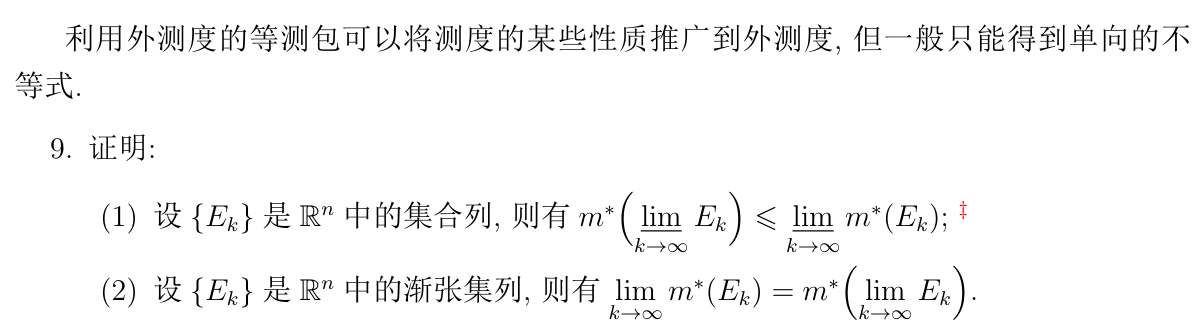
\includegraphics[width=\textwidth]{hw6-2025041611.png}
% \caption{}
\label{}
\end{figure}
\end{exercise}
\begin{proof}
(1) 对每个 $E_k$ 作等测包 $H_k$ 满足
\[
E_k\subset H_k,\qquad m^{*}E_k=mH_k
\]
从而
\[
m^{*}(\varliminf_{ k \to \infty } E_k)\overset{ E_k\subset H_k }{ \leq  }\underbrace{ m^{*}(\varliminf_{ k \to \infty } H_k) }_{ =m(\varliminf_{ k \to \infty } H_k) }=\varliminf_{ k \to \infty } mH_k=\varliminf_{ k \to \infty } m^{*}E_k
\]
(2) 由于 $E_k\uparrow$, 所以 $E_1\subset E_2\subset\dots \subset E_k\subset\dots$. 从而
\[
\varlimsup_{ k \to \infty } E_k=\bigcap_{k=1}^{\infty}\underbrace{ \bigcup_{n=k}^{\infty} E_n }_{ =\bigcup_{n=k+1}^{\infty} E_n }=\bigcup_{n=1}^{\infty} E_k
\]
\[
\varliminf_{ k \to \infty } E_k=\bigcup_{k=1}^{\infty} \underbrace{ \bigcap_{n=k}^{\infty} E_n }_{ =E_k }=\bigcup_{k=1}^{\infty} E_k=\varlimsup_{ k \to \infty } E_k
\]
因此 $\lim_{ k \to \infty }E_k$ 存在. 由 (1) 可知:
\[
m^{*}(\lim_{ k \to \infty } E_k)\leq \lim_{ k \to \infty } m^{*}E_k
\]
同时,因为 $E_k\subset \lim_{ k \to \infty }E_k=\bigcup_{k=1}^{\infty}E_k,\forall k\geq1$,所以
\[
m^{*}E_k\leq  m^{*}(\lim_{ k \to \infty } E_k)\qquad \forall k\geq 1
\]
因此
\[
\lim_{ k \to \infty } m^{*}E_k\leq m^{*}(\lim_{ k \to \infty } E_k)
\]
故
\[
\lim_{ k \to \infty } m^{*}E_k=m^{*}(\lim_{ k \to \infty } E_k)
\]
\end{proof}

\begin{exercise}
\begin{figure}[H]
\centering
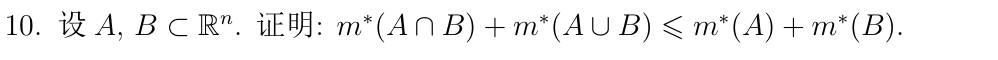
\includegraphics[width=\textwidth]{1-hw6-2025041611.png}
% \caption{}
\label{}
\end{figure}
\end{exercise}
\begin{proof}
设 $H_1,H_2$ 分别是 $A,B$ 的等测包,那么
\[
mH_1+mH_2=m(H_1\cap H_2)+m(H_1\cap H_2^{c})+mH_2
\]
由于
\[
H_1\cap H_2^{c}\cap H_2=\varnothing
\]
\[
(H_1\cap H_2^{c})\cup H_2=(H_1\cup H_2)\cap(\underbrace{ H_2^{c}\cup H_2 }_{ =\mathbb{R}^{n} })=H_1\cup H_2
\]
从而
\[
mH_1+mH_2=m(H_1\cap H_2)+m(H_1\cup H_2)
\]
由于 $A\subset H_1,B\subset H_2$,所以
\[
A\cap B\subset H_1\cap H_2,\qquad A\cup B\subset H_1\cup H_2
\]
因此
\[
m^{*}(A\cap B)\leq m(H_1\cap H_2),\qquad m^{*}(A\cup B)\leq m(H_1\cup H_2)
\]
从而
\[
\begin{aligned}
m^{*}(A\cap B)+m^{*}(A\cup B) & \leq m(H_1\cap H_2)+m(H_1\cup H_2) \\
 & =mH_1+mH_2 \\
 & =m^{*}A+m^{*}B
\end{aligned}
\]
\end{proof}

\begin{exercise}
\begin{figure}[H]
\centering
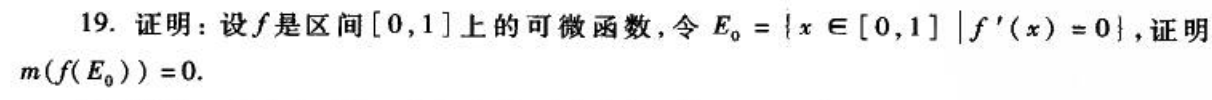
\includegraphics[width=\textwidth]{hw6-2025041612.png}
% \caption{}
\label{}
\end{figure}
\end{exercise}
\begin{note}
\begin{figure}[H]
\centering
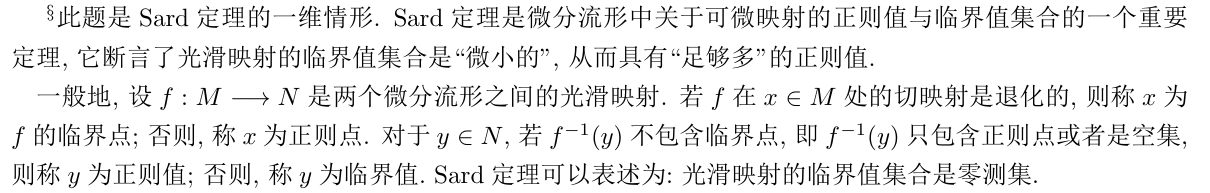
\includegraphics[width=\textwidth]{1-hw6-2025041612.png}
% \caption{}
\label{}
\end{figure}
\end{note}
\begin{figure}[H]
\centering
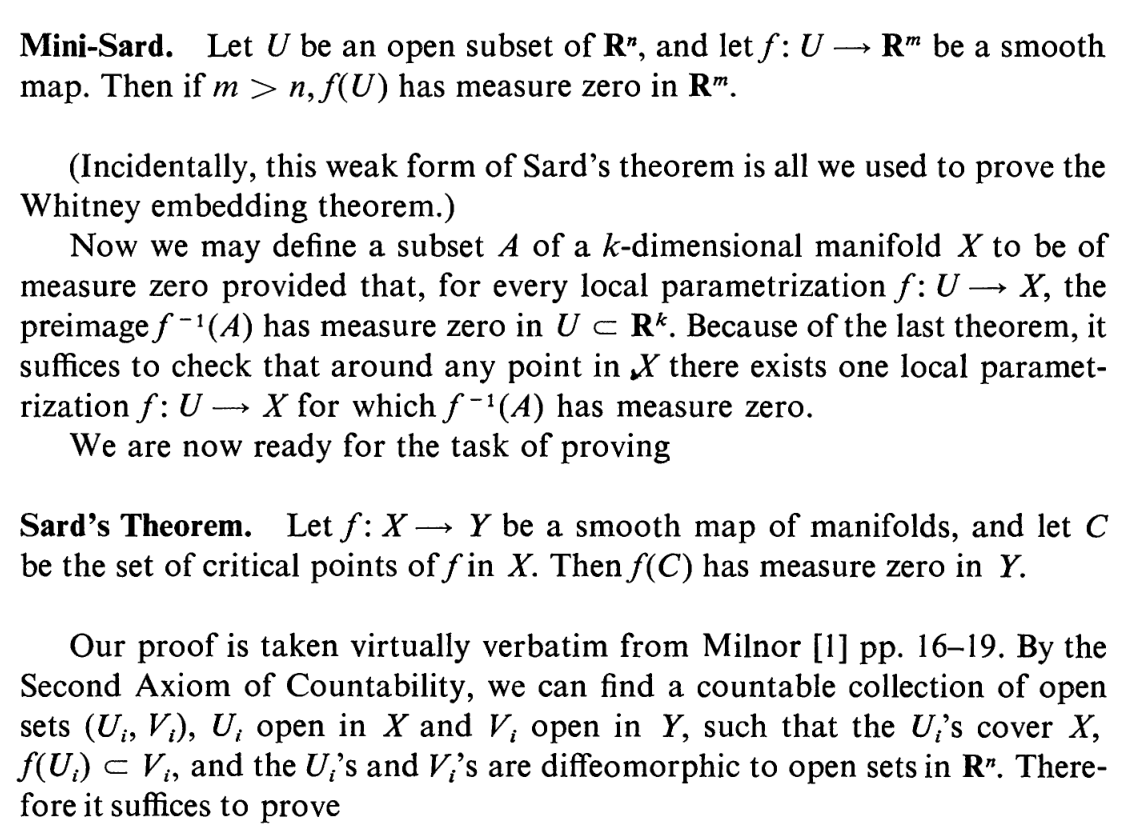
\includegraphics[width=\textwidth]{2-hw6-2025041612.png}
% \caption{}
\label{}
\end{figure}
\begin{figure}[H]
\centering
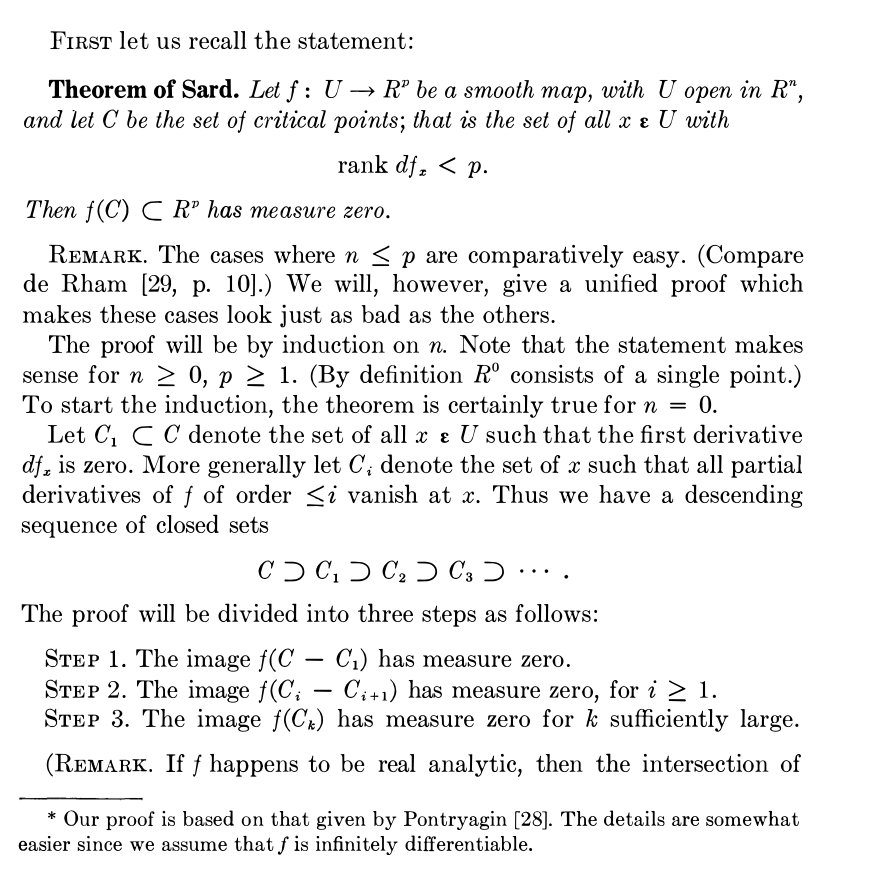
\includegraphics[width=\textwidth]{3-hw6-2025041612.png}
% \caption{}
\label{}
\end{figure}
\begin{figure}[H]
\centering
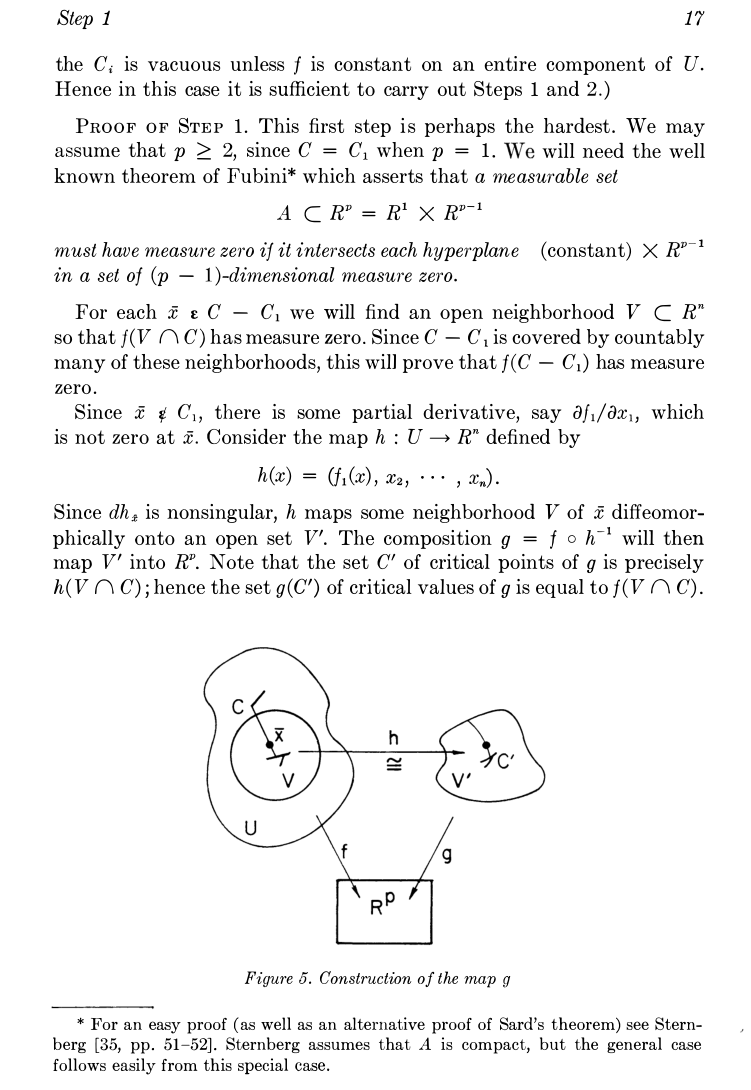
\includegraphics[width=\textwidth]{4-hw6-2025041612.png}
% \caption{}
\label{}
\end{figure}
\begin{figure}[H]
\centering
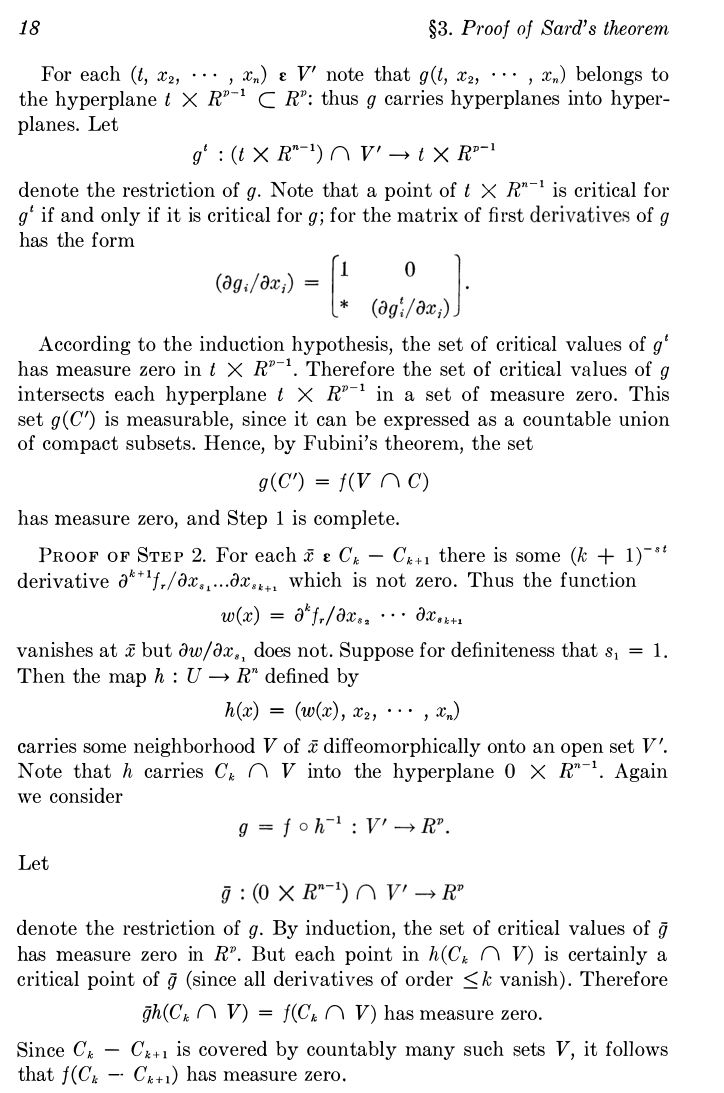
\includegraphics[width=\textwidth]{5-hw6-2025041612.png}
% \caption{}
\label{}
\end{figure}
\begin{figure}[H]
\centering
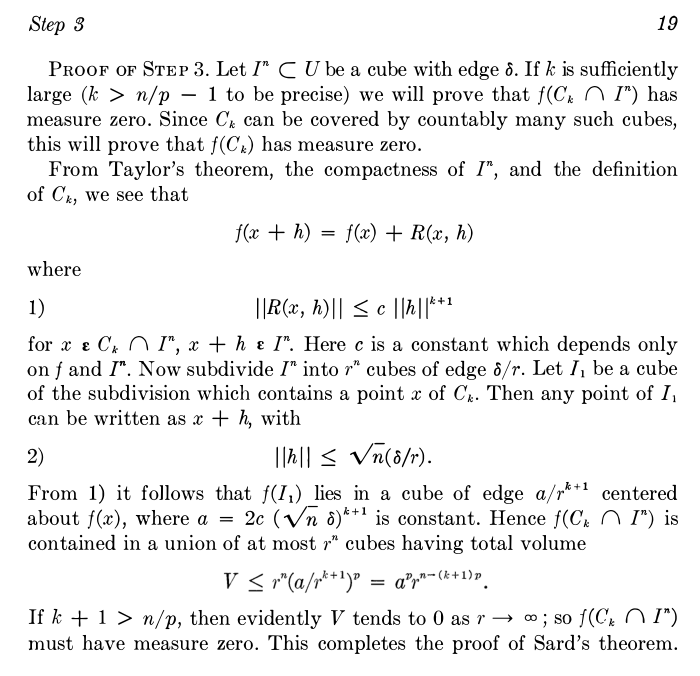
\includegraphics[width=\textwidth]{6-hw6-2025041612.png}
% \caption{}
\label{}
\end{figure}

\begin{exercise}
\begin{figure}[H]
\centering
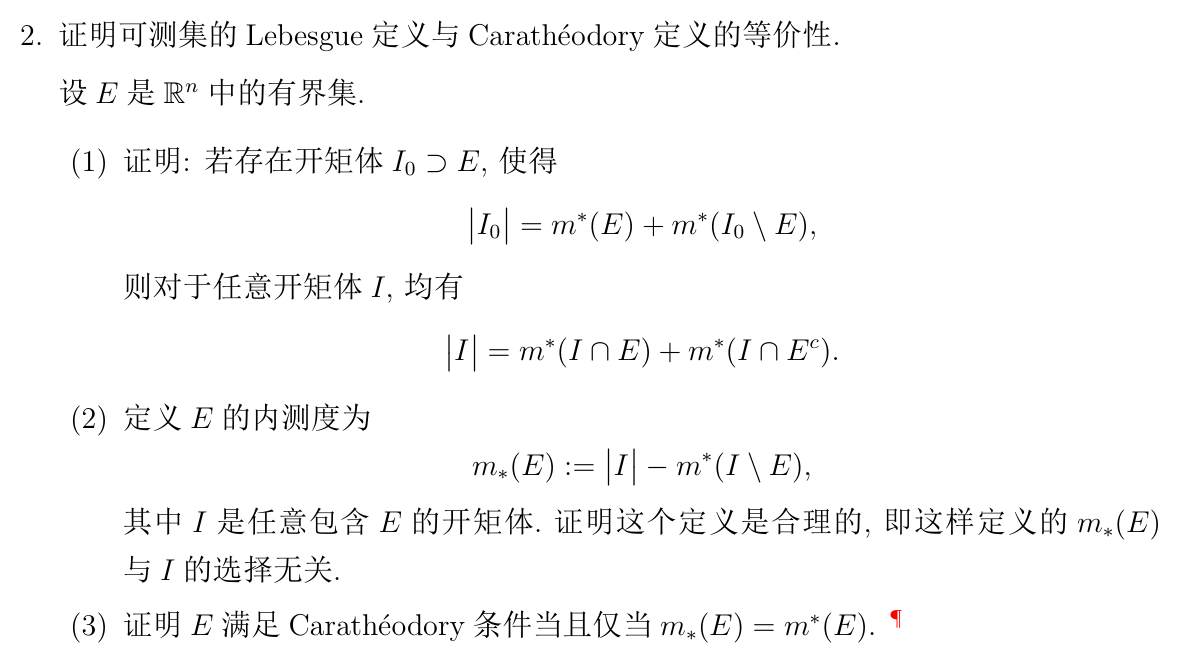
\includegraphics[width=\textwidth]{7-hw6-2025041612.png}
% \caption{}
\label{}
\end{figure}
\end{exercise}